\documentclass[]{article}

\usepackage{graphicx}

\usepackage[margin=1in]{geometry}

\setlength\parindent{0pt}

\usepackage{physics}
\usepackage{amsmath, amsfonts, amssymb, amsthm}

\usepackage{listings}

\usepackage{enumitem}
\renewcommand{\theenumi}{\alph{enumi}}
\renewcommand*{\thesection}{Problem \arabic{section}}
\renewcommand*{\thesubsection}{\alph{subsection})}
\renewcommand*{\thesubsubsection}{\quad \quad \roman{subsubsection})}

%Custom Commands
\newcommand{\Rel}{\mathcal{R}}
\newcommand{\R}{\mathbb{R}}
\newcommand{\C}{\mathbb{C}}
\newcommand{\N}{\mathbb{N}}
\newcommand{\Z}{\mathbb{Z}}
\newcommand{\Q}{\mathbb{Q}}

\newcommand{\toI}{\xrightarrow{\textsf{\tiny I}}}
\newcommand{\toS}{\xrightarrow{\textsf{\tiny S}}}
\newcommand{\toB}{\xrightarrow{\textsf{\tiny B}}}

\newcommand{\divisible}{ \ \vdots \ }
\newcommand{\st}{ \ \vline \ }


% Theorem Definition
\newtheorem{definition}{Definition}
\newtheorem{assumption}{Assumption}
\newtheorem{theorem}{Theorem}


%opening

\title{MATH 5301 Elementary Analysis - Midterm Exam}

\author{Jonas Wagner}

\date{2021, October 8}

\begin{document}

\maketitle

% Problem 1
\section{}
\textbf{Problem:} 100 soldiers stayed in a rank in front of the corporal. 
The corporal ordered all of them to turn left, but the soldiers were newbies, 
so they were not certain was it left from their perspective or from the corporal’s 
point of view. So, some of them turned left and some turned right. After that 
at every second if two neighboring soldiers find themselves facing each other,
they rotate by 180 degrees. Show that this process will not last forever.

\subsection*{Problem Formulation}
The state of the 100 soldiers represented as arrows pointed to the right or left 
for each time step, $n$, is visualized by the following drawing:\\
\begin{figure}[h]
    \centering
    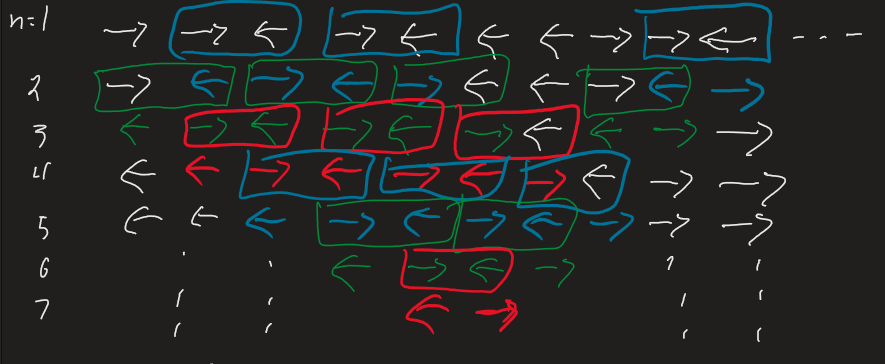
\includegraphics[width=0.7\textwidth]{MidExam1_pblm1_a.png}
\end{figure}

For each time step all of the individual pairs of soldiers facing each other 
flip and it progresses until all soldiers on the left face left and soldiers 
on the right face right.\\

This can be similarly described as a sequence of binary states and a simplistic update 
operation.\\
Let $1$ denote $\rightarrow$.\\
Let $0$ denote $\leftarrow$.\\
Define and randomly populate sequence 
$$\qty{x_n \st x_n \in \{0,1\} }_{n \in [1,100]}^{(k)}, k \in \N$$
The dependent update operation can be defined as 
$$\qty{x_n}^{(k+1)} 
    := \qty{x_n \st x_n = 
    \begin{cases}
        1   & (x_n \land x_{n+1}) \lor (~x_n \land x_{n-1})\\
        0   & (~x_n \land ~x_{n-1}) \lor (x_n \land ~x_{n+1})
    \end{cases}
    \
    }
$$
where $x_0 = 0$ and $x_{101} = 1$ get referenced.\\

\newpage
\subsection*{Stopping Demonstration}
An example demonstrating this progression on the left is shown in the following drawing: 
\begin{figure*}[h]
    \centering
    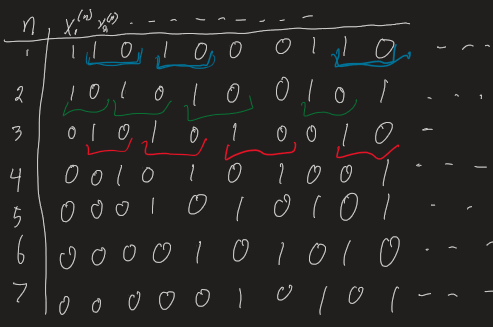
\includegraphics[width = 0.7 \textwidth]{MidExam1_pblm1_b.png}
\end{figure*}

It is clear that after each update, the system will begin to converge so that 
$$\exists_{a \in [1,100]} : \forall_{i < a} x_i = 0$$ and 
$$\exists_{b \in [1,100]} : \forall_{i > b} x_i = 1$$

Therefore, and since $\qty{x_n}^{(k)}$ is a finite set, the following must be true:
$$\exists_{n \in \N} \forall_{k > n} \implies \qty{X_n}^{(k)} = \qty{X_n}^{(k+1)}$$

Which means that the dependent operation will no longer change the state of the system.

% Problem 2
\newpage
\section{}
Let $\R^\infty$ be the set of all sequences of real numbers
$$\R^\infty = \qty{a_1,a_2,\cdots \ | \ a_j \in \R}$$
Define the relation $\Rel$ on $\R^\infty$ as follows:
$a\Rel b$ if for some $j \in \N : a_j > b_j$ and for all $k < j \implies a_k = b_k$.


Does it mean this?
$$\exists_{j \in \N} : \qty((a_j > b_j) \land (\forall_{k<j} \implies a_k = b_k))$$
or this?
$$\qty(\exists_{j \in \N} : (a_j > b_j \land \forall_{k<j})) \implies a_k = b_k$$

Prove that such a relation is an order relation on $R^\infty$. Is it a total order?



$$\exists_{j\in\N} : \qty(\forall_{k < j} \ a_k = b_k) \land (a_j > b_j)$$










% Problem 3
\newpage
\section{}
Alice wrote some finite sequence of zeros and ones on the paper (e.g. 010010). 
Bob is allowed to replace any pair ``10'' by ``00···01'' with any (but finite) 
amount of zeros in front of 1. Bob can repeat this procedure as many times as 
he wants (if he will find ``10'' in the resulting sequence). 
Prove that Bob can perform such operation only finitely many times.













% Problem 4
\newpage
\section{}
Present two essentially different total orderings of the field 
$\Q(\sqrt{2}) := \qty{a + b \sqrt{2} \st a,b \in \Q}$.
\subsection*{Problem Formulation}
\begin{definition}
    The field $\mathbb{F} = \langle\Q(\sqrt{2}),+,0,\cdot,1\rangle$ is defined with the set
    $$\Q(\sqrt{2}) := \qty{a + b \sqrt{2} \st a,b \in \Q}$$
    and the operators
    \begin{align*}
        + : \Q(\sqrt{2}) \cross \Q(\sqrt{2}) \to \Q(\sqrt{2}) 
            &:= (a_1,a_2) + (b_1,b_2) = (a_1 + b_1, a_2 + b_2)\\
        \cdot : \Q(\sqrt{2}) \cross \Q(\sqrt{2}) \to \Q(\sqrt{2}) 
            &:= (a_1,a_2) \cdot (b_1,b_2) = (a_1 b_1 + 2 a_2 b_2, a_1 b_2 + a_2 b_1)
    \end{align*}
    It is also assumed that the standard field properties all apply.
\end{definition}


This is not good... need to fix it....:

% % Part 1
% \subsection{Ordering 1: $\Rel_1$}
% \begin{definition}
%     An relation $a \Rel_1 b$ %$(a,b) \Rel_1 (b_1,b_2)$ can be defined as
%     $$\Rel \subset \Q(\sqrt{2}) \cross \Q(\sqrt{2}) 
%         := \qty{(a,b) \st a \cdot a \leq b \cdot b}$$
% \end{definition}
% \begin{theorem}
%     The relation $a \Rel_1 b$ is an ordered relation over $\mathbb{F}$
%     \begin{proof}
%         Over $\mathbb{F}$ the ordered relation $(a_1,a_2) \Rel_1 (b_1,b_2)$ can be defined by 
%         $$(a, b) \Rel_1 (b_1,b_2) 
%             := \qty{((a_1,a_2),(b_1,b_2)) \st (a_1 \cdot a_1 + 2 \cdot a_2 \cdot a_2) 
%                 \leq (b_1 \cdot b_1 + 2 \cdot b_2 \cdot b_2)}
%         $$
%         $(a_1, a_2) \Rel_1 (b_1,b_2)$ satisfies the 3 ordered properties:
%         \subsubsection{Reflective: $x \Rel_1 x$}
%         \begin{align*}
%             (a_1 \cdot a_1 + 2 \cdot a_2 \cdot a_2) 
%                 \leq (b_1 \cdot b_1 + 2 \cdot b_2 \cdot b_2)
%                 &\implies a \Rel_1 b\\
%             (x_1 \cdot x_1 + 2 \cdot x_2 \cdot x_2) 
%                 \leq (x_1 \cdot x_1 + 2 \cdot x_2 \cdot x_2)
%                 &\implies x \Rel_1 x\\
%             x_1^2 + 2 x_2^2 \leq x_1^2 + 2 x_2^2 &\implies x \Rel_1 x
%         \end{align*}
        
%         \subsubsection{Anti-Symmetry: $x \Rel_1 y \land y \Rel_1 x \implies x = y$}
%         \begin{align*}
%             x \Rel_1 y \land y \Rel_1 x &\implies x = y\\
%             (x_1,x_2) \Rel_1 (y_1,y_2) \land (y_1,y_2) \Rel_1 (x_1,x_2) 
%                 &\implies (x_1,x_2)=(y_1,y_2)\\
%             \qty((x_1 \cdot x_1 + 2 \cdot x_2 \cdot x_2)
%                     \leq (y_1 \cdot y_1 + 2 \cdot y_2 \cdot y_2))
%             &\land\\
%                 \land \qty((y_1 \cdot y_1 + 2 \cdot y_2 \cdot y_2)
%                     \leq (x_1 \cdot x_1 + 2 \cdot x_2 \cdot x_2))
%                 &\implies (x_1,x_2) = (y_1,y_2)\\
%             \qty(x_1^2 + 2 x_2^2 \leq y_1^2 + 2 y_2^2)
%                 \land \qty(y_1^2 + 2 y_2^2 \leq x_1^2 + 2 x_2^2)
%                 &\implies (x_1,x_2) = (y_1,y_2)\\
%             % (x \cdot x \leq y \cdot y) \land (y \cdot y \leq x \cdot x)
%             %     &\implies x = y
%         \end{align*}
        
%         \subsubsection{Transivity: $x \Rel_1 y \land y \Rel_1 z \implies x \Rel_1 z$}
%         \begin{align*}
%             x \Rel_1 y \land y \Rel_1 z 
%                 &\implies x \Rel_1 z\\
%             (x_1,x_2) \Rel_1 (y_1,y_2) \land (y_1,y_2) \Rel_1 (z_1,z_2)
%                 &\implies (x_1,x_2) \Rel_1 (z_1,z_2)\\
%             \qty((x_1 \cdot x_1 + 2 \cdot x_2 \cdot x_2)
%                     \leq (y_1 \cdot y_1 + 2 \cdot y_2 \cdot y_2)) 
%                 \land&\\
%                 \land \qty((y_1 \cdot y_1 + 2 \cdot y_2 \cdot y_2)
%                     \leq (z_1 \cdot z_1 + 2 \cdot z_2 \cdot z_2)) 
%                 &\implies \qty((x_1 \cdot x_1 + 2 \cdot x_2 \cdot x_2)
%                     \leq (z_1 \cdot z_1 + 2 \cdot z_2 \cdot z_2))\\
%             \qty(x_1^2 + 2 x_2^2 \leq y_1^2 + 2 y_2^2)
%                     \land \qty(y_1^2 + 2 y_2^2 \leq z_1^2 + 2 z_2^2)
%                 &\implies \qty(x_1^2 + 2 x_2^2 \leq z_1^2 + 2 z_2^2)\\
%             x_1^2 + 2 x_2^2 \leq y_1^2 + 2 y_1^2 \leq z_1^2 + 2 z_2^2
%                 &\implies x \Rel_1 z
%         \end{align*}
%     \end{proof}
% \end{theorem}
% \begin{theorem}
%     The ordered relation $x \Rel_1 y$ forms a total order over $\mathbb{F}$.
%     \begin{proof}
%         $x \Rel_1 y$ satisfies the totality condition:
%         \subsubsection{Totality: 
%         $\forall x,y \in \mathbb{F} \implies x \Rel_1 y \lor y \Rel_1 x$}
%         \begin{align*}
%             \forall x,y \in \mathbb{F} &\implies x \Rel_1 y \lor y \Rel_1 x\\
%             \forall_{x \in \Q(\sqrt{2})}
%                     \forall_{y \in \Q(\sqrt{2})}
%                 &\implies \qty(x \cdot x \leq y \cdot y)
%                     \lor \qty(y \cdot y \leq x \cdot x)\\
%             \forall_{(x_1,x_2) \in \Q(\sqrt{2}))}
%                     \forall_{(y_1,y_2) \in \Q(\sqrt{2})}
%                 &\implies \qty((x_1 \cdot x_1 + 2 \cdot x_2 \cdot x_2)
%                     \leq (y_1 \cdot y_1 + 2 \cdot y_2 \cdot y_2)) \lor\\
%                 &\qquad \lor \qty((y_1 \cdot y_1 + 2 \cdot y_2 \cdot y_2)
%                     \leq (x_1 \cdot x_1 + 2 \cdot x_2 \cdot x_2))\\
%             % \forall_{x_1 \in \N} \forall_{x_2\in \N}
%             %         \forall_{y_1 \in \N} \forall_{y_2 \in \N}
%             \forall_{x_1, x_2, y_1, y_2 \in \Q}
%                 &\qty(\qty(x_1^2 + 2 x_2^2 \leq y_1^2 + 2 y_2^2)
%                     \lor \qty(y_1^2 + 2 y_2^2 \leq x_1^2 + 2 x_2^2))\\
%             % \forall_{x_1, x_2, y_1, y_2 \in \Q(\sqrt{2})}
%             %     &\qty(x_1^2 + 2 x_2^2 \leq y_1^2 + 2 y_2^2)
%             %         \lor \qty(y_1^2 + 2 y_2^2 \leq x_1^2 + 2 x_2^2)
%         \end{align*}
%     \end{proof}
% \end{theorem}

% % Part 2
% \subsection{Ordering 2: $\Rel_2$}
% \begin{definition}
%     An relation $a \Rel_2 b$
%     $$\Rel \subset \Q(\sqrt{2}) \cross \Q(\sqrt{2}) 
%         := \qty{(a,b) \st a \cdot a \leq b \cdot b}$$
% \end{definition}


% % not done yet
% \begin{theorem}
%     The relation $a \Rel_1 b$ is an ordered relation over $\mathbb{F}$
%     \begin{proof}
%         Over $\mathbb{F}$ the ordered relation $(a_1,a_2) \Rel_1 (b_1,b_2)$ can be defined by 
%         $$(a, b) \Rel_1 (b_1,b_2) 
%             := \qty{((a_1,a_2),(b_1,b_2)) \st (a_1 \cdot a_1 + 2 \cdot a_2 \cdot a_2) 
%                 \leq (b_1 \cdot b_1 + 2 \cdot b_2 \cdot b_2)}
%         $$
%         $(a_1, a_2) \Rel_1 (b_1,b_2)$ satisfies the 3 ordered properties:
%         \subsubsection{Reflective: $x \Rel_1 x$}
%         \begin{align*}
%             (a_1 \cdot a_1 + 2 \cdot a_2 \cdot a_2) 
%                 \leq (b_1 \cdot b_1 + 2 \cdot b_2 \cdot b_2)
%                 &\implies a \Rel_1 b\\
%             (x_1 \cdot x_1 + 2 \cdot x_2 \cdot x_2) 
%                 \leq (x_1 \cdot x_1 + 2 \cdot x_2 \cdot x_2)
%                 &\implies x \Rel_1 x\\
%             x_1^2 + 2 x_2^2 \leq x_1^2 + 2 x_2^2 &\implies x \Rel_1 x
%         \end{align*}
        
%         \subsubsection{Anti-Symmetry: $x \Rel_1 y \land y \Rel_1 x$}
%         \begin{align*}
%             x \Rel_1 y \land y \Rel_1 x &\implies x = y\\
%             (x_1,x_2) \Rel_1 (y_1,y_2) \land (y_1,y_2) \Rel_1 (x_1,x_2) 
%                 &\implies (x_1,x_2)=(y_1,y_2)\\
%             \qty((x_1 \cdot x_1 + 2 \cdot x_2 \cdot x_2)
%                     \leq (y_1 \cdot y_1 + 2 \cdot y_2 \cdot y_2))
%             &\land\\
%                 \land \qty((y_1 \cdot y_1 + 2 \cdot y_2 \cdot y_2)
%                     \leq (x_1 \cdot x_1 + 2 \cdot x_2 \cdot x_2))
%                 &\implies (x_1,x_2) = (y_1,y_2)\\
%             \qty(x_1^2 + 2 x_2^2 \leq y_1^2 + 2 y_2^2)
%                 \land \qty(y_1^2 + 2 y_2^2 \leq x_1^2 + 2 x_2^2)
%                 &\implies (x_1,x_2) = (y_1,y_2)\\
%             % (x \cdot x \leq y \cdot y) \land (y \cdot y \leq x \cdot x)
%             %     &\implies x = y
%         \end{align*}
        
%         \subsubsection{Transivity: $x \Rel_1 y \land y \Rel_1 z \implies x \Rel_1 z$}
%         \begin{align*}
%             x \Rel_1 y \land y \Rel_1 z 
%                 &\implies x \Rel_1 z\\
%             (x_1,x_2) \Rel_1 (y_1,y_2) \land (y_1,y_2) \Rel_1 (z_1,z_2)
%                 &\implies (x_1,x_2) \Rel_1 (z_1,z_2)\\
%             \qty((x_1 \cdot x_1 + 2 \cdot x_2 \cdot x_2)
%                     \leq (y_1 \cdot y_1 + 2 \cdot y_2 \cdot y_2)) 
%                 \land&\\
%                 \land \qty((y_1 \cdot y_1 + 2 \cdot y_2 \cdot y_2)
%                     \leq (z_1 \cdot z_1 + 2 \cdot z_2 \cdot z_2)) 
%                 &\implies \qty((x_1 \cdot x_1 + 2 \cdot x_2 \cdot x_2)
%                     \leq (z_1 \cdot z_1 + 2 \cdot z_2 \cdot z_2))\\
%             \qty(x_1^2 + 2 x_2^2 \leq y_1^2 + 2 y_2^2)
%                     \land \qty(y_1^2 + 2 y_2^2 \leq z_1^2 + 2 z_2^2)
%                 &\implies \qty(x_1^2 + 2 x_2^2 \leq z_1^2 + 2 z_2^2)\\
%             x_1^2 + 2 x_2^2 \leq y_1^2 + 2 y_1^2 \leq z_1^2 + 2 z_2^2
%                 &\implies x \cdot x \leq y \cdot y \leq z \cdot z
%         \end{align*}
%     \end{proof}
% \end{theorem}

% \begin{theorem}
%     The ordered relation $x \Rel_1 y$ forms a total order over $\mathbb{F}$.
%     \begin{proof}
%         $x \Rel_1 y$ satisfies the totality condition:
%         \subsubsection{Totality: 
%         $\forall x,y \in \mathbb{F} \implies x \Rel_1 y \lor y \Rel_1 x$}
%         \begin{align*}
%             \forall x,y \in \mathbb{F} &\implies x \Rel_1 y \lor y \Rel_1 x\\
%             \forall_{x \in \Q(\sqrt{2})}
%                     \forall_{y \in \Q(\sqrt{2})}
%                 &\implies \qty(x \cdot x \leq y \cdot y)
%                     \lor \qty(y \cdot y \leq x \cdot x)\\
%             \forall_{(x_1,x_2) \in \Q(\sqrt{2}))}
%                     \forall_{(y_1,y_2) \in \Q(\sqrt{2})}
%                 &\implies \qty((x_1 \cdot x_1 + 2 \cdot x_2 \cdot x_2)
%                     \leq (y_1 \cdot y_1 + 2 \cdot y_2 \cdot y_2)) \lor\\
%                 &\qquad \lor \qty((y_1 \cdot y_1 + 2 \cdot y_2 \cdot y_2)
%                     \leq (x_1 \cdot x_1 + 2 \cdot x_2 \cdot x_2))\\
%             % \forall_{x_1 \in \N} \forall_{x_2\in \N}
%             %         \forall_{y_1 \in \N} \forall_{y_2 \in \N}
%             \forall_{x_1, x_2, y_1, y_2 \in \N}
%                 &\qty(\qty(x_1^2 + 2 x_2^2 \leq y_1^2 + 2 y_2^2)
%                     \lor \qty(y_1^2 + 2 y_2^2 \leq x_1^2 + 2 x_2^2))\\
%             % \forall_{x_1, x_2, y_1, y_2 \in \Q(\sqrt{2})}
%             %     &\qty(x_1^2 + 2 x_2^2 \leq y_1^2 + 2 y_2^2)
%             %         \lor \qty(y_1^2 + 2 y_2^2 \leq x_1^2 + 2 x_2^2)
%         \end{align*}
%     \end{proof}
% \end{theorem}






% Problem 5
\newpage
\section{}
Infinitely many wizards $W_1, W_2,\dots$ stay in the line.
Each wizard wears a hat of one the three colors: Red, Yellow or Green. 
Every wizard $W_n$ can see the hats of all the next wizards in line, $W_{n+1}, W_{n+2}, \dots$,
Starting  with  the  wizard $W_1$ every one has to guess the color of his own hat. 
If the wizard guesses correctly, he can go free. Otherwise he got dematerialized. 
Wizards  discussed  their  strategy  before  this  event. 
Show that if the wizards were smart enough, then only finitely many of them will disappear.

\subsection*{Assumptions}
\begin{assumption}\label{asmp:selfless}
    It is assumed that the Wizards are not only all smart, but also selfless to attempt to 
    save the most number of wizards instead of just themselves.
\end{assumption}
\begin{assumption}
    Although it is not stated in the problem, it is assumed that the Wizards 
    are unable to directly communicate the color of the hats to someone else, 
    but it is also assumed that an infinite memory of past guesses exists.
\end{assumption}

\subsection*{Sequence Definitions}
\begin{definition}
    Let the sequence $\qty{W_n}$ be defined as
    $$\qty{W_n} := \qty{W_n \st W_n \in \{1,2,3\}}$$
    with index $n$ related to each of the wizards in order and 
    $1,2,3$ represent `Red', `Yellow', and `Green' respectively.
\end{definition}
\begin{definition}
    Let the updating sequence $\qty{G_n}$ be defined as the guess that each Wizard makes.
\end{definition}
\begin{definition}
    An updating sequence $\qty{Q_n}$ is defined as a queue of causal memory that each wizard 
    maintains according to the same set of rules.
\end{definition}
\subsection*{Decision Procedure}
The procedure described is one of many potential decision criterion that can be used to 
make guesses and minimize the number of incorrect hat color guesses. The basic idea 
is that following the initialization of the procedure, each Wizard will maintain their own 
queue based on what previous Wizards guessed and what they perceive from the following 
Wizards hat colors. This queue will be long enough that when a wizard is reached it should 
know what color their own hat is along with future hat colors. They then make a decision based 
on the queue and the wizard following the end of the queue as to what hat to guess in order 
to either share information to the future Wizards or to save themselves. The procedure is 
designed so that repeated colors are used to expand the length of the queue and allow 
for wizards to use the information to save themselves without creating a deficit.
By Assumption \ref{asmp:selfless}, the decision will always be according to the procedure 
that will do the best for everyone and not just save themselves.

\newpage
The following pseudo-code outlines the decision procedure that all the wizards will use. 
Let $N=\infty$, time index $n$, queue length $k$, and arbitrarily set minimum queue length $K = 20$.
\begin{lstlisting}
% Initialization
for i = 5:N % min start is 5
    if W(i+1) == W(i) % First set of same color hat
        k = i;
        break
    end
end
% Initialize Queue
for n = 1:k
    G(n) = W(n + k);
    Q(n + k) = G(n);
end
% Standard Decision Procedure
while n < N
    if Q(n) == Q(n+1)
        G(n) = Q(n);
    else if k > K && G(n) ~= W(n+k)
        G(n) = Q(n);
    else
        G(n) = W(n + k)
        Q(n + k) = G(n);
    end
    while W(n + k) == W(n + k + 1)
        Q(n + k + 1) = W(n + k + 1);
        k = k + 1;
    end
    n = n + 1;
end
\end{lstlisting}
% look at that else if statement again... and make sure it'll still work


\subsection*{Effectiveness of Procedure}
A proof of Effectiveness is probably easily demonstrated through mathematical induction. 
Essentially, the finite loss of Wizards can be demonstrated using the size of $k$ 
being bounded from below and increasing regardless of the color of the next hat.
% Demonstrate with actual things...





% Problem 6
\newpage
\section{}
Show that $A$ is an infinite set if and only if $A$ has a proper subset 
$B \ : \ (B \subsetneq A)$ with the same cardinality $(\abs{A} = \abs{B})$.






\end{document}
